% Copyright (C) 2013 Columbia University in the City of New York and others.
%
% Please see the AUTHORS file in the main source directory for a full list
% of contributors.
%
% This file is part of TerraFERMA.
%
% TerraFERMA is free software: you can redistribute it and/or modify
% it under the terms of the GNU Lesser General Public License as published by
% the Free Software Foundation, either version 3 of the License, or
% (at your option) any later version.
%
% TerraFERMA is distributed in the hope that it will be useful,
% but WITHOUT ANY WARRANTY; without even the implied warranty of
% MERCHANTABILITY or FITNESS FOR A PARTICULAR PURPOSE. See the
% GNU Lesser General Public License for more details.
%
% You should have received a copy of the GNU Lesser General Public License
% along with TerraFERMA. If not, see <http://www.gnu.org/licenses/>.

\chapter{Incompressible Laminar Plumes: \citeauthor{VattevilleG32009}} \label{sec:vatteville}

\citet{VattevilleG32009} performed laboratory experiments where 
a thermal plume was initiated from a circular heater 
in a square tank of silicone oil at several heater
powers.  Approximating the domain to be cylindrically symmetric, they
demonstrated that the experimental results could be reproduced 
by finite element modeling in axisymmetric cylindrical geometry.

Using the same cylindrical approximation we examine four cases, at
different heater power levels (0.6, 1.0, 1.7 and \W[3.3]). Boundary
conditions are chosen to mimic those of the laboratory tank: no--slip
conditions are specified on the bottom (including the heater) and the
external side of the domain, while free--slip and no normal flow
conditions are specified at the top and internal side, $r=0$. For
temperature, the external wall and top boundary are kept at room
temperature. The bottom boundary is also held at room temperature,
except at the heater itself, where we prescribe the measured
time--dependent evolution of heater temperature, from the laboratory
experiments (this is available along with other model parameters in
\citet{VattevilleG32009}). Homogeneous Neumann conditions are
specified on the internal wall.  Adaptive time-stepping targets a
maximum Courant number of $2.5$.

The  model incorporates a temperature dependent viscosity law:
\begin{align}
\mu =& \exp\left(b_0 + \frac{b_1}{T_i+\Delta T}\right), % \\
\end{align}

Results are presented in the Figure \ref{fig:vatteville}. In Figure
\ref{fig:vatteville}(a), we plot the maximum velocity along the plume
conduit, as a function of time, for the experimental data and simulation results. 
The experimentally measured
velocity field is slightly noisy, due to the statistical nature of
Particle Image Velocimetry (PIV), but compares quantitatively well
with the velocity field predicted by \TF{}, over a range of supplied
powers and, hence, over a range of heater temperatures. We
consistently observe that the near--steady plume conduit velocity
predicted numerically is higher than the laboratory
measurements. Identical discrepancies were observed between the
numerical and laboratory results of \citet{VattevilleG32009}.

One critical aspect of the laboratory measurements is that the PIV
method uses an averaging window that is necessary to compile
statistically meaningful velocities \citep[see][for further
details]{VattevilleG32009}. To mimic the effects of this averaging, we
post--process numerical results by averaging in \mm[3] squares over
the domain.  
% PvK: not really.... This mimics the laser sheet used for the PIV measurements
%in the experiments.  
% mspieg: Okay...how do you want to fix this (or is it okay for the
% current purposes)
Averaging has the effect of reducing the
discrepancy between experimentally sampled and numerically predicted
velocities (Figure \ref{fig:vatteville}).

\begin{figure}[htb]
\begin{tabular}{cc}
\footnotesize (a) Peak velocities & \footnotesize (b) Velocity profiles (\W[1.0] heater) \vspace{0.3cm} \\
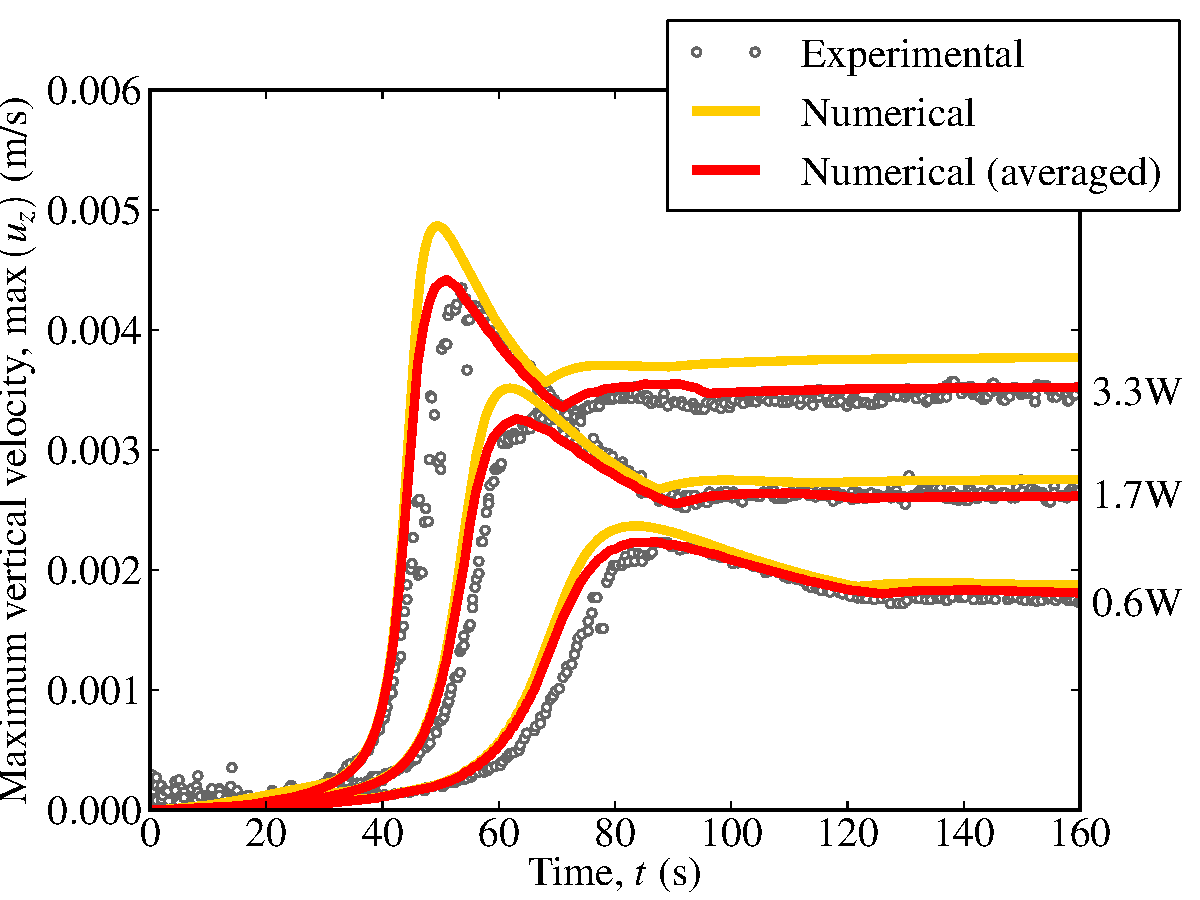
\includegraphics[width=0.47\textwidth]{data/vatteville/max_velocity} & 
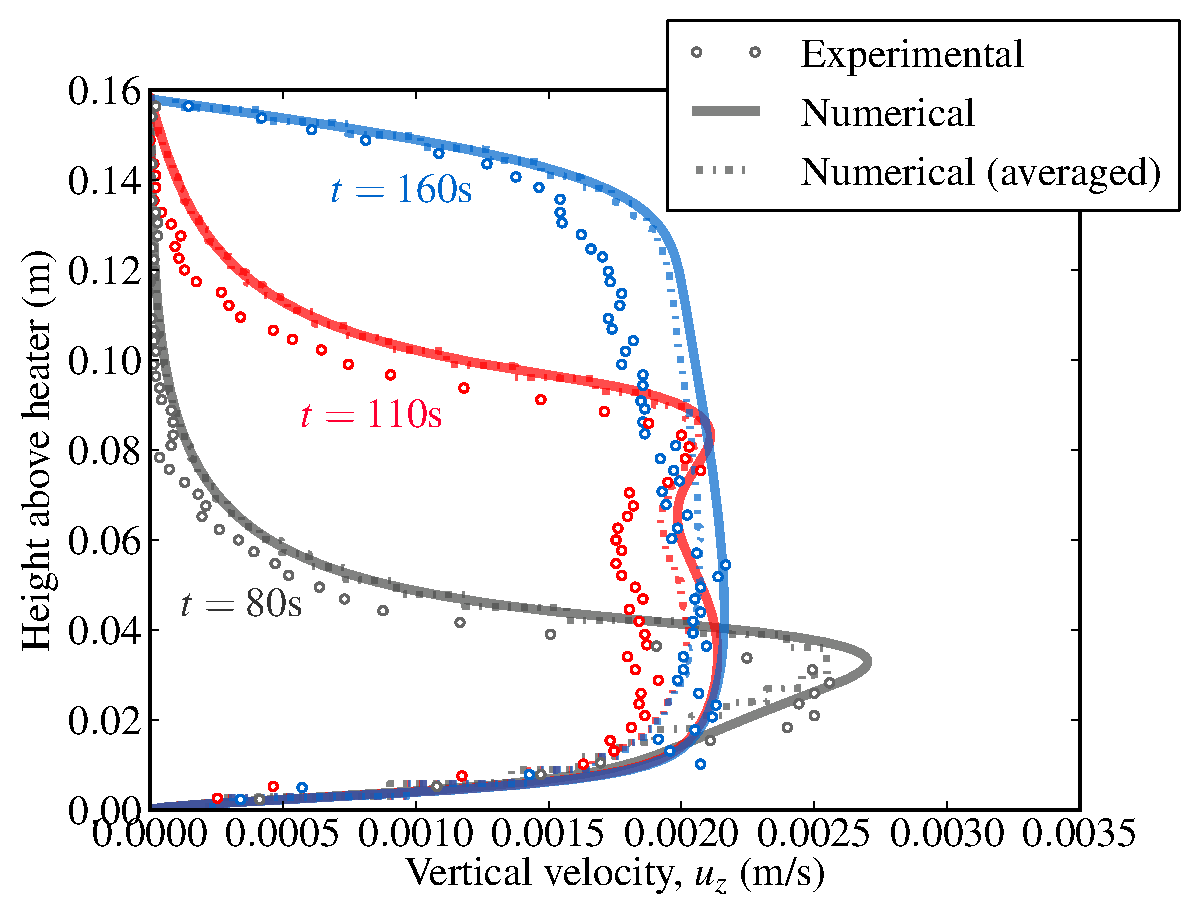
\includegraphics[width=0.47\textwidth]{data/vatteville/velocity_profile} \vspace{0.2cm} \\
\end{tabular}
\caption{(a) Benchmark results for \cite{VattevilleG32009} showing maximum velocities versus time in the laboratory experiments  and
the numerical simulations for a cylindrical plume.  Following \citet{VattevilleG32009}, the numerical data is averaged in \mm[3] squares to mimic the effect of laboratory data collection.  The effect of this averaging can also be seen in velocity profiles of the numerical 
and laboratory data above the heater (b, heater power of \W[1.0]).} 
\label{fig:vatteville}
\end{figure}



